\documentclass{report}
\usepackage[utf8]{inputenc}
\usepackage[margin=20mm]{geometry}
\usepackage{graphicx}
\graphicspath{ {./img/} }
\usepackage{amsmath}
\usepackage{amssymb}
\usepackage{tabularx}
\usepackage{subcaption}
\usepackage{float}
\usepackage{titlesec}
\usepackage{enumitem}
\usepackage{multicol}
\usepackage{amsthm}
\renewcommand*\contentsname{Indice}

% El psy kongroo
% Definizione di un ambiente per i teoremi
\newtheorem{teorema}{Teorema}
\newtheorem{definizione}{Definizione}

% Definire lo stile per le sezioni e sottosezioni
\titleformat{\section}[block]
  {\normalfont\fontsize{20}{24}\bfseries\filcenter} % Font size and style
  {\thesection}{10pt}{} % Section number format

\titleformat{\subsection}[block]
  {\normalfont\fontsize{15}{18}\bfseries} % Font size and style
  {\thesubsection}{10pt}{} % Subsection number format

% Rimuovere l'indentazione a sinistra dei titoli delle sezioni e sottosezioni
\titlespacing*{\section}{0pt}{*2}{*1.5}
\titlespacing*{\subsection}{0pt}{*1.5}{*1}


% Gap righe
\renewcommand{\arraystretch}{1.6}


\title{Basi di dati Appunti\\ -\\ secondo parziale}
\author{Dimitri}
\date{A.A. 2024/2025}

\begin{document}
\maketitle
\newpage
\tableofcontents
\newpage
%sezione non completa

\chapter{Algebra Relazionale}
\section{Introduzione}
L'algebra relazionale è un linguaggio procedurale formale di tipo algebrico i cui operandi sono relazioni.
Questo linguaggio non è usato nelle implementazioni dei vari DBMS ma definisce in maniera semplice tutte le operazioni tipiche dei diversi linguaggi di interrogazione.
Da un punto di vista didattico l’algebra relazionale è utile perché essendo svincolata dai “dettagli
implementativi” dell’SQL (o di altri linguaggi), permette di comprendere rapidamente la tecnica d’uso dei linguaggi di interrogazione per basi di dati relazionali.\\
\section{Operatori}
\subsection{Introduzione}
In Algebra relazionale è possibile classificare i diversi operatori in base alla derivabilità oppure in modo funzionale. Questi operatori possono essere binari o unari, e tramite questi ultimi vengono descritte le procedure di interrogazione.\\
Nella classificazione in base alla derivabilità si distiguono 6 operatori di base e diversi derivati:\\
\textbf{Operatori di Base:}
\begin{itemize}
    \item Selezione
    \item Proiezione
    \item Ridenominazione
    \item Unione
    \item Differenza
    \item Prodotto cartesiano
\end{itemize}
\textbf{Operatori derivati:}
\begin{itemize}
    \item Intersezione
    \item Join
\end{itemize}
\newpage
\subsection{Selezione $\sigma$}
La selezione è un'operazione unaria. Seleziona le tuple di una relazione che soddisfano un predicato producendo un sottoinsieme delle stesse, (ossia seleziona le righe della tabella che rispettano la condizione data, ricordiamo che con tuple si intendono le righe della tabella mentre con attributi le singole colonne).\\
Lo schema della relazione risultato è lo stesso di quella di origine ed il predicato è costituito dal nome di un attributo, da un operatore, e da un altro argomento che può essere un attributo o un valore
costante.\\
$$\sigma_{\text{predicato}}(relazione)$$\\
La cardinalità di questa operazione è la seguente:\\
$$ 0 \leq |\sigma_{\text{F}}(R)| \leq |R|$$\\

\subsection{Proiezione $\Pi$}
La proiezione è un'operazione unaria. Data una relazione, la sua proiezione su un dato insieme di attributi è costituita dalla tabella generata dagli attributi specificati, contenente tutte le tuple della tabella di partenza, (ossia estrae tutte le colonne corrispondenti alla lista di attributi specificati).\\
$$\Pi_{\text{lista attributi}}(relazione)$$\\
La cardinalità di questa operazione è la seguente:\\
$$min(|R|, 1) \leq \Pi_{\text{y}}(R) \leq |R|$$\\

\subsection{Ridenominazione $\rho$}
A volte in preparazione all’esecuzione di una interrogazione o in seguito ad una sua esecuzione si ha bisogno di rinominare gli attributi di una relazione. A tal fine l’operatore di ridenominazione che permette di ottenere una nuova tabella con i nuovi nomi per gli attributi modificati e che ha le stesse tuple della tabella originale.\\
$$\rho_{\text{vecchio nome $\to$ nuovo nome}}(relazione)$$\\

\subsection{Unione $\cup$}
L’unione fra due tabelle è rappresentata da una tabella costituita dall’unione “matematica” delle due tabelle, dove quindi sono presenti le tuple della prima tabella e quelle della seconda. Affinché l’unione abbia senso, è necessario che:
\begin{itemize}
    \item le due tabelle abbiano lo stesso numero di attributi;
    \item i tipi degli attributi corrispondenti siano uguali;
\end{itemize}
Se il numero degli attributi delle due relazioni (tabelle) non è uguale, si genera un errore.\\
La cardinalità di questa operazione è la seguente:\\
$$max(|R1|, |R2|) \leq |R1 \cup R2| \leq |R1| + |R2|$$\\

\subsection{Differenza -}
La differenza fra due tabelle A e B è una tabella che contiene le tuple che sono presenti in A ma non in
B. Come nel caso dedll'unione, questa operazione può essere eseguita solo se le relazioni hanno lo stesso grado (numero di colonne) e gli attributi sono compatibili.\\
La cardinalità di questa operazione è la seguente:\\
$$0 \leq |R1 - R2| \leq |R1|$$\\

\subsection{Prodotto Cartesiano $\times$}
Il prodotto cartesiano fra due tabelle è una tabella con schema la somma degli schemi, se due attributi
sono uguali questi sono ripetuti le tuple della tabella sono il risultato del prodotto cartesiano dei suoi elementi, ossia da tutte le coppie possibili composte dagli elementi appartenenti alle due relazioni.\\
$$R1\times R2$$\\
La cardinalità di questa operazione è la seguente (ricordiamo che se il Join è completo il limite inferiore diventa $max(|R1|,|R2|)$):\\
$$|R1 \times R2| = |R1| \cdot |R2|$$\\

\subsection{Intersezione $\cap$}
Il risultato dell'operazione di intersezione tra due relazioni è una relazione contenente le tuple che appartengono ad entrambe le relazioni, anche in questo caso valgono le stesse condizioni di unione e differenza per la validità dell'operazione.\\
$$R1 \cap R2$$\\
La cardinalità di questa operazione è la seguente:\\
$$ 0 \leq |R1 \cap R2| \leq min(|R1|, |R2|)$$\\

\section{Join}
\subsection{Introduzione}
E’ l’operatore più caratteristico dell’algebra relazionale, in quanto è quello che permette di correlare dati contenuti in relazioni diverse confrontando i valori comuni contenuti in esse.\\
Esistono diverse varianti di tale operatore comunque riconducibili l’una con l’altra:
\begin{itemize} 
    \item Join Naturale
    \item Join Esterni
    \item Theta Join ed Equi Join\\
\end{itemize}
\subsection{Join Naturale $\bowtie$}
Il Join naturale è un operatore binario che correla dati in relazioni diverse sulla base dei valori uguali in attributi con lo stesso nome. La relazione risultante è una tabella che ha come attributi l’unione degli attributi delle tabelle iniziali e contiene solamente le tuple che hanno valori uguali negli attributi in comune.\\
Quando non si hanno attributi comuni il join naturale diventa un prodotto cartesiano, perch\'e genera tutte le possibili coppie. 

\paragraph{Esempio.}  Prendiamo lo schema: \\

\noindent\texttt{DOCENTE(\underline{CFDocente}, Nome, Cognome) \\
CORSO(\underline{Nome}, CFDocente)}\\

\noindent Si richiede di produrre l'insieme dei corsi riportando: nome del corso e cognome del docente.
\[ \Pi_{\text{NomeCorso, Cognome}}(\rho_{\text{Nome $\to$ NomeCorso}}(CORSO) \bowtie \thickspace DOCENTE)\]
Graficamente si ottiene:

\begin{center}
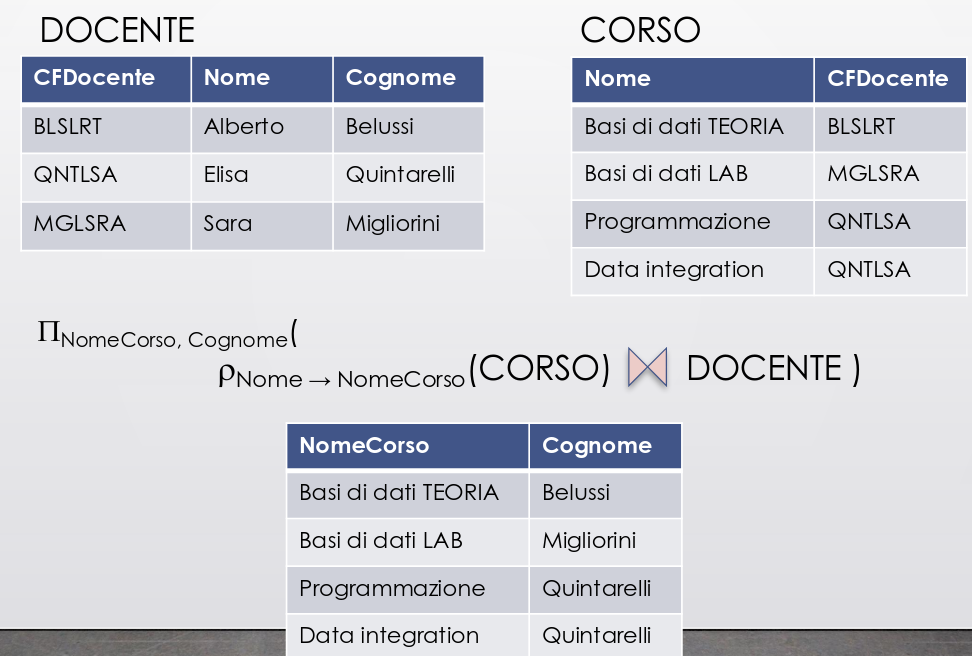
\includegraphics[scale=0.35]{join_example}
\end{center}


Il Join può essere ottenuto tramite un prodotto cartesiano e una selezione imponendo l’uguaglianza su tutti gli attributi in comune:\\
\[\sigma_{\text{NomeCorso = Nome}}(DOCENTE \times CORSO)\]
Il Join si dice completo se ogni tupla della relazione A contribuisce a generare almeno una tupla della relazione risultato, altrimenti si dice incompleto e le tuple che non contribuiscono al risultato si chiamano \textbf{dangling tuples}.

La cardinalità del Join Naturale è, in generale:
\[0 \leq |R1 \bowtie R2| \leq |R1| \cdot |R2|\]
Se il join \`e completo la cardinalit\`a diventa:
\[ max(|R1|, |R2|) \leq |R1 \bowtie R2| \leq |R1| \cdot |R2| \]
Se $X_1 \cap X_2$ \`e una superchiave per $R2$:
\[ 0 \le |R1 \bowtie R2| \leq |R1| \]
Il caso pi\`u classico che ricounduce a questa situazione \`e quando si fa l'uguaglianza tra una \emph{chiave} e una \emph{chiave esportata}, ovvero abbiamo esportato la chiave di $R2$ su $R1$. Se prendo una tupla di $R1$ che ha tra i suoi attributi una \emph{superchiave} di $R2$, si avr\`a al massimo una tupla di $R2$ che va in combinazione con la tupla di partenza di $R1$, perci\`o, \emph{al massimo} la cardinalit\`a sar\`a quella di $R1$. Se $X_1 \cap X_2$ \`e una superchiave di $R2$ ed esiste un \emph{vincolo di integrit\`a referenziale} tra $X_1 \cap X_2$, o una parte di $R1$, e $R2$: $|R1 \bowtie R2| = |R1|$.

\subsection{Theta join ed equi-join}
Nel theta join il predicato di join viene esplicitato, \`e indipendente dallo schema.
Date le relazioni $R1$ e $R2$, rispettivamente di schema $X_1$ e $X_2$, la \textbf{precondizione} al theta join \`e che gli schemi di $R1$ e $R2$ devono essere \emph{disgiunti}: $X_1 \cap X_2 = \varnothing $.
\[ R1 \bowtie_{\theta} R2 = \sigma_{\theta}(R1 \bowtie R2) \]
Dove il join naturale all'interno della selezione funge da \emph{prodotto cartesiano} e $\theta$ \`e un predicato conforme alla sintassi prevista per l'operatore di selezione.
\subsubsection{Esempio}
\texttt{DOCENTE(\underline{CF}, Nome, Cognome)\\
CORSO(\underline{Nome}, Docente)\\
}
Si richiede di produrre l'elenco di tutti i corsi riportando: nome del corso e cognome del docente.
\[ \Pi_{\text{NomeCorso, Cognome}}(\rho_{\text{Nome $\to$ NomeCorso}}(CORSO) {\Large \bowtie \atop \text{\tiny{CF = Docente}}} DOCENTE) \]
Graficamente:
\begin{center}
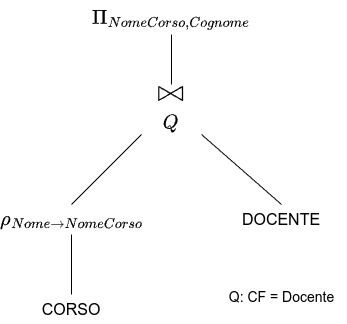
\includegraphics[scale=0.5]{theta_join_example}
\end{center}

\subsubsection{Equi-join}
Il theta join si dice \emph{equi-join} se la condizione $\theta$ \`e una congiunzione di uguaglianze:
\[ R1 {\bowtie \atop A_1 = B_1 \wedge \dots \wedge A_n = B_n} R2 \]

Si noti che \textbf{non esiste} un operatore misto che applica la logica del join naturale per gli attributi comuni e aggiunge la condizione specificata esplicitamente attraverso il predicato $\theta$.

\subsubsection{Propriet\`a dell'equi-join}

Date due relazioni $R1$ e $R2$ di schema $X_1$ e $X_2$, con $X_1 \cap X_2 = \{ C_1, \dots, C_m\}$ con $m > 0$, vale la seguente equivalenza:
\[ R1 \bowtie R2 = \Pi_{X_1 \cup X_2} \left(R1 {\bowtie \atop C_1=C_1' \wedge \dots \wedge C_m=C_m'} \rho_{C_1,\dots,C_m \to C_1', \dots, C_m'}(R2)\right) \]
In questo caso si hanno due relazioni che hanno attributi comuni ($\{ C_1, \dots, C_m\}$) e quindi si devono ridenominare gli attributi di una delle due relaizoni, nell'esempio quelli di $R2$. A questo punto gli schemi sono disgiunti e la condizione del theta-join sar\`a una congiunzione di uguaglianze: $C_1=C_1' \wedge \dots \wedge C_m=C_m'$. Gli attributi che si ottengono nel risultato del theta-join sono la somma degli attributi di $R1$ e di $R2$, cosa che non avviene nel join naturale. Per questo motivo si proietta su $\Pi_{X_1\cup X_2}$, in questo modo l'unione considera gli attributi di tutte e due le relazioni ma esclude i $C_1', \dots, C_m'$ generati nell'espressione.

\subsection{Join esterni}
Consentono di ottenere nel risultato del join tutte le tuple, anche le \textbf{dangling tuples}, di una o di entrambe le relazioni coinvolte nel join, eventualmente estese con valori nulli:
\begin{itemize}
	\item \textbf{left join}: $r_1 \bowtie_{LEFT} r_2$;
	\item \textbf{right join}: $r_1 \bowtie_{RIGHT} r_2$;
	\item \textbf{full join}: $r_1 \bowtie_{FULL} r_2$;
\end{itemize}

\section{Ottimizzazione}
\subsection{Valori nulli}
E’ opportuno estendere l’algebra relazionale affinché possa manipolare anche relazioni che contengono \emph{valori nulli} (NULL). Le operazioni che devono essere raffinate per gestire relazioni che contengono valori nulli sono in particolare \textbf{selezione} e \textbf{join naturale}.\\
Le altre operazioni riportano semplicemente nelle tuple del risultato il valore nullo presente sulle tuple di input.

\subsubsection{Selezione}
Nel caso della \textbf{selezione} abbiamo che la selezione applicata a:
\begin{itemize}
\item $A \theta B$ risulta essere falsa (quindi non seleziona quella determinata tupla) se uno dei due attributi A o B è NULL.
\item $A \theta const$ risulta essere falsa se l'attributo $A$ \`e NULL.
\end{itemize}
Inoltre, si aggiungono le seguenti condizioni atomiche:
\begin{itemize}
\item \texttt{A IS NULL}: \`e una condizione atomica che viene valutata sulla tupla $t$. \`E \textbf{vero} se $t[A]$ \emph{contiene} il valore NULL, altrimenti \`e \textbf{falso}. 
\item \texttt{A IS NOT NULL}: \`e una condizione atomica che viene valutata sulla tupla $t$. \`E \textbf{vero} se $t[A]$ \emph{\underline{non} contiene} il valore NULL, altrimenti \`e \textbf{falso}.
\end{itemize}

\subsubsection{Join naturale}
La condizione di uguaglianza sugli attributi comuni alle due relazioni \`e \textbf{falsa} sulle tuple $t_1$ e $t_2$ se almeno uno degli attributi comuni di $t_1$ o di $t_2$ \`e NULL. Inoltre, il confronto particolare $NULL = NULL$ \`e \textbf{sempre valutato FALSO}.

\subsection{Ottimizzatore}
Ogni espressione DML\footnote{Solitamente specificata in linguaggio dichiarativo} ricevuta dal DBMS viene sottoposta ad un processo di elaborazione, tra cui, anche uno di ottimizzazione. L’ottimizzatore genera un’espressione equivalente all’interrogazione di input e di costo inferiore. quest'ultimo viene valutato in termini di \textbf{dimensione dei risultati intermedi}.
L’ottimizzatore esegue \textbf{trasformazioni di equivalenza} allo scopo di riddurre la dimensione dei risultati intermedi.

\subsubsection{Equivalenza tra espressioni algebriche}

\paragraph{Equivalenza dipendente dallo schema.} Dato uno schema $R$:
$E_1 \equiv E_2$ se $E_1(r) = E_2(r)$ per ogni istanza di $r$ di schema $R$.\\
Esempio:
\[ \Pi_{AB}(R_1) \bowtie \Pi_{AC}(R_2) \equiv_R \Pi_{ABC}(R_1 \bowtie R_2) \]
Con $R=\{R_1(A, B, D), R_2(A, C, E)\}$.

La condizione generale che lo schema deve soddisfare \`e che l'\textbf{unico attributo comune tra $R_1$ e $R_2$ sia $A$}.

\paragraph{Equivalenza assoluta.} \`E indipendente dallo schema.

$E_1 \equiv E_2$ se $E_1 \equiv_R E_2$ per ogni schema $R$ compatibile con $E_1$ ed $E_2$.\\
Esempio:
\[ \Pi_{AB}(\sigma_{A>0}(R_1)) \equiv \sigma_{A>0}(\Pi_{AB}(R1))\]


\subsubsection{Trasformazioni di equivalenza}
Le principali trasformazioni sono quattro. Consideriamo, per gli esempi, il seguente schema relazionale:\\
\texttt{
TRENO(\underline{NumTreno}, OrarioPart, Cat, Dest, OrarioArr)\\
FERMATA(\underline{NumTreno, Stazione}, Orario)
}

Sia $E$ un'espressione di schema $X$, si definiscono le seguenti trasformazioni di equivalenza:
\begin{itemize}
    \item \textbf{Atomizzazione delle selezioni:} una congiunzione di selezioni può essere sostituita da una sequenza di selezioni atomiche.
\[ \sigma_\text{F1 $\wedge$ F2}(E) \equiv \sigma_\text{F1}(\sigma_\text{F2}(E))\] \`E propedeutica ad altre trasformazioni. Non ottimizza se non \`e seguita da altre trasformazioni. \\
Esempio:
\[ \Pi_{\text{NumTreno, OrarioPart}}(\sigma_{\text{Cat='FR' $\wedge$ Stazione='Vicenza'}}(TRENO \bowtie FERMATA) \]
\[ \Large \Rightarrow \]
\[ \Pi_{\text{NumTreno, OrarioPart}}(\sigma_{\text{Cat='FR'}}(\sigma_{\text{Stazione='Vicenza'}}(TRENO \bowtie FERMATA))) \]
\begin{multicols}{2}[Graficamente:]

\begin{center}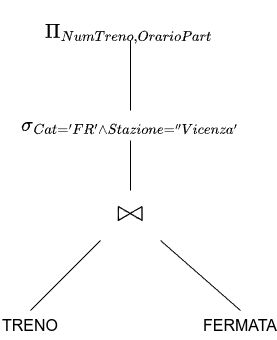
\includegraphics[scale=0.45]{tree_example_transform}\end{center}
\begin{center}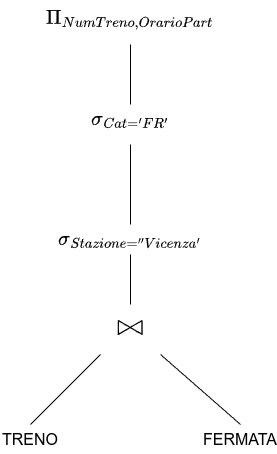
\includegraphics[scale=0.45]{tree_example_atomizz_sel}\end{center}
\end{multicols}
    \item \textbf{Idempotenza delle proiezioni:} una proiezione può essere trasformata in una sequenza di proiezioni che eliminano i vari attributi in varie fasi.
\[ \Pi_\text{A}(E) \equiv \Pi_\text{A}(\Pi_\text{A,B}(E)) \text{ dove }B \subseteq X \]
\`E propedeutica ad altre trasformazioni. Non ottimizza se non \`e seguita da altre trasformazioni. 
\end{itemize}
\newpage
Siano $E_1$ ed $E_2$ espressioni di schema $X_1$ e $X_2$, si definiscono le seguenti trasformazioni di equivalenza:
\begin{itemize}
    \item \textbf{Anticipazione della selezione rispetto al join:} questa espressione vale solo se $F$ conivolge \textbf{solo} gli attributi di $E_2$.
\[ \sigma_{F}(E_1 \bowtie E_2) \equiv_R E_1 \bowtie \sigma_{F}(E_2) \]

Esempio:
\[ \Pi_{\text{NumTreno, OrarioPart}}(\sigma_{\text{Cat='FR' $\wedge$ Stazione='Vicenza'}}(TRENO \bowtie FERMATA) \]
\[ \Large \Rightarrow \]
\[ \Pi_{\text{NumTreno, OrarioPart}}(\sigma_{\text{Cat='FR'}}(TRENO)) \bowtie \sigma_{\text{Stazione='Vicenza'}}(FERMATA)) \]
\begin{multicols}{2}[Graficamente:]

\begin{center}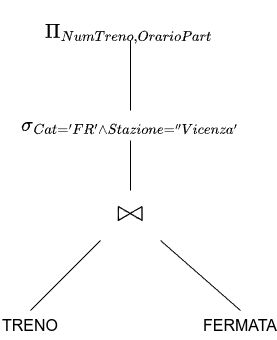
\includegraphics[scale=0.45]{tree_example_transform}\end{center}
\begin{center}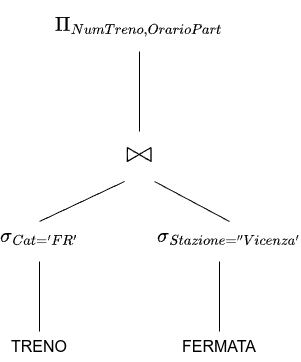
\includegraphics[scale=0.45]{tree_example_anticip_sel}\end{center}
\end{multicols}

    \item \textbf{Anticipazione della proiezione rispetto al Join:} vale solo se Y sono attributi di B e I suoi attributi sono coinvolti nel join.\\
\[\Pi_\text{Y}(A \bowtie B) \equiv A \bowtie(\Pi_\text{Y}(B))\]
Esempio:
\[ \Pi_{\text{NumTreno, OrarioPart}}(\sigma_{\text{Cat='FR' $\wedge$ Stazione='Vicenza'}}(TRENO \bowtie FERMATA) \]
\[ \Large \Rightarrow \]
\[ \Pi_{\text{NumTreno, OrarioPart}}(\Pi_{\text{NumTreno, OrarioPart}}(\sigma_{\text{Cat='FR'}}(TRENO)) \bowtie \Pi_{\text{NumTreno}}(\sigma_{\text{Stazione='Vicenza'}}(FERMATA)) \]
\begin{multicols}{2}[Graficamente:]

\begin{center}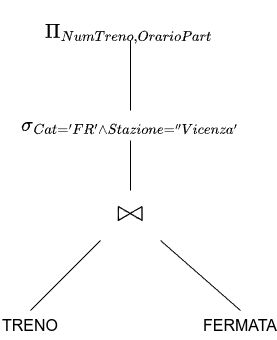
\includegraphics[scale=0.45]{tree_example_transform}\end{center}
\begin{center}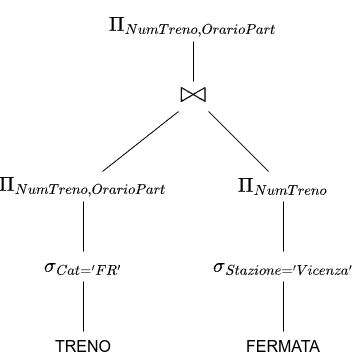
\includegraphics[scale=0.45]{tree_example_anticip_projection}\end{center}
\end{multicols}

    \item Esistono poi altre otimizzazioni minori come l'inglobamento di una selezione in un join (da eseguire solo se non è possibile anticipare la selezione), in questo caso la condizione di selezione sarà assorbita nel \textbf{theta-join}.\\
$$\sigma_\text{F}(A \bowtie B) \equiv A \bowtie_\text{F} B$$
    Infine è bene ricordare anche le trasformazioni con gli operatori insiemistici:\\
$$\sigma_\text{F or G}(A) \equiv \sigma_\text{F}(A) \cup \sigma_\text{G}(A)$$
$$\sigma_\text{F and G}(A) \equiv \sigma_\text{F}(A) \cap \sigma_\text{G}(A)$$
    
\end{itemize}



\newpage
\chapter{Calcolo Relazionale}

\end{document}
